\chapter{Metodología}	
\label{ch:metodología}

Este capítulo explica cómo se ha organizado el trabajo, qué decisiones se han tomado en cada etapa y, en particular, por qué. Se han seguido ---con cierta libertad--- las líneas de la metodología CRISP-DM~\cite{wirth2000crisp}, que resulta adecuada para estructurar un proyecto de este tipo, aunque en la práctica el proceso fue menos lineal de lo que el diagrama sugiere.

\section{El marco CRISP-DM}

CRISP-DM (Cross Industry Standard Process for Data Mining) es una metodología que propone seis fases iterativas. En la práctica el ciclo rara vez se sigue de forma estricta ---el avance entre fases no es lineal y se producen retrocesos frecuentes---, pero proporciona un marco conceptual útil. La Figura~\ref{fig:crisp_dm} ilustra las fases.

\begin{figure}[H]
\centering
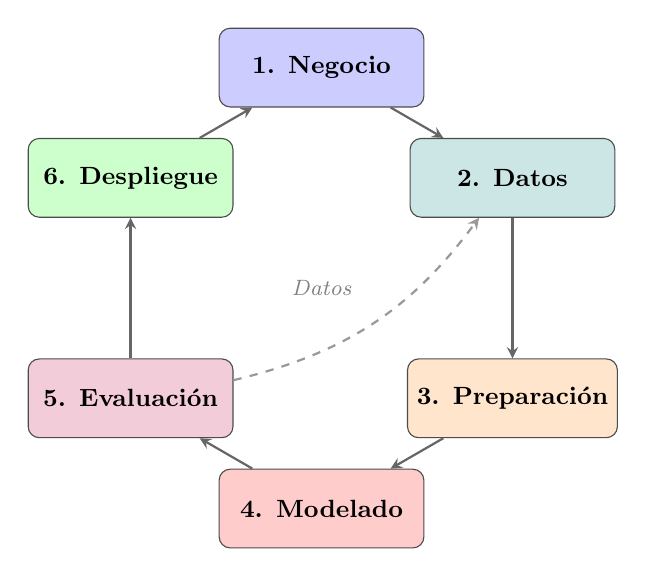
\begin{tikzpicture}[
  phase/.style={rectangle, rounded corners=4pt, draw=black!70, fill=#1!20,
    minimum width=2.6cm, minimum height=1cm, text centered, font=\small\bfseries},
  arr/.style={->, >=stealth, thick, draw=black!60},
  every node/.style={font=\small}
]
  % Nodos en disposición hexagonal
  \node[phase=blue]   (n) at (90:2.8)  {1. Negocio};
  \node[phase=teal]   (d) at (30:2.8)  {2. Datos};
  \node[phase=orange] (p) at (330:2.8) {3. Preparación};
  \node[phase=red]    (m) at (270:2.8) {4. Modelado};
  \node[phase=purple] (e) at (210:2.8) {5. Evaluación};
  \node[phase=green]  (dp) at (150:2.8){6. Despliegue};
  % Centro
  \node[font=\footnotesize\itshape, text=black!50] at (0,0) {Datos};
  % Flechas del ciclo
  \draw[arr] (n)  -- (d);
  \draw[arr] (d)  -- (p);
  \draw[arr] (p)  -- (m);
  \draw[arr] (m)  -- (e);
  \draw[arr] (e)  -- (dp);
  \draw[arr] (dp) -- (n);
  % Retroalimentación hacia datos (línea punteada)
  \draw[arr, dashed, black!40] (e) to[bend right=20] (d);
\end{tikzpicture}
\caption{Fases del proceso CRISP-DM aplicadas al proyecto.}
\label{fig:crisp_dm}
\end{figure}

\section{El punto de partida}

El trabajo parte de una pregunta de investigación: ¿mejora la predicción del precio de cierre la incorporación de una señal de sentimiento de mercado? Para responderla se requieren datos fiables, modelos de distinta complejidad y un protocolo de evaluación que respete la causalidad temporal.

La selección de activos buscó deliberadamente perfiles distintos. BTC-USD se incluyó por su elevada volatilidad y porque cotiza las 24~horas~\cite{corbet2019cryptocurrencies}. Las dos acciones tecnológicas (TSLA y NVDA) añaden puntos de comparación con dinámicas diferentes: ambas tienen alta cobertura mediática, pero por razones distintas.

TSLA resulta relevante por la fuerte influencia que las declaraciones públicas de su CEO ejercen sobre su cotización, y NVDA, por su exposición directa a los ciclos del sector de IA y semiconductores, con fluctuaciones notables en los últimos años.

\section{Los datos}

\subsection{Precios históricos}

Los datos de precios vienen de Yahoo Finance, vía la librería yfinance. Es una fuente gratuita y suficientemente fiable para un trabajo de fin de grado. Se descargaron datos diarios desde noviembre de 2020 hasta noviembre de 2025; el dataset útil empieza en enero de 2021 porque los primeros meses se emplean en el cálculo de indicadores técnicos y en la alineación del sentimiento.

Para mejorar la reproducibilidad y evitar discontinuidades artificiales en acciones (por ejemplo, por \textit{splits}), en la descarga se emplea la opción \texttt{auto\_adjust=True} de yfinance, de forma que las series OHLC quedan ajustadas.

Cada observación incluye apertura, máximo, mínimo, cierre y volumen (OHLCV). Para el modelado se utiliza principalmente el precio de cierre, mientras que los indicadores técnicos se calculan a partir de la serie disponible.

\subsection{Datos de sentimiento}

Para el sentimiento se recurrió a GDELT~\cite{gdelt2024api}, que cubre los tres activos. A partir del \textit{Average Tone} se construyó una serie diaria filtrando noticias que mencionan Bitcoin, Tesla o Nvidia (con consultas tipo \texttt{(Bitcoin OR BTC)}, etc.). Como medida complementaria se añadió el \textit{Volume Intensity}, que refleja cuánta cobertura recibe cada activo. Esta fuente tiene la ventaja de ser gratuita, sin límites estrictos de cuota y con un histórico largo.

Esta elección aporta coherencia: en vez de usar un proxy genérico de sentimiento de mercado, la señal está ligada directamente a cada activo. Constituye un enfoque más riguroso para contrastar la hipótesis de que el contenido informativo específico de un activo añade algo que no está ya en sus precios pasados~\cite{baker2007investor}.

\subsection{Preparación de los datos}

Los datos crudos no se pueden utilizar directamente ---se requiere un preprocesado sustancial---. Lo primero fue alinear temporalmente precios y sentimiento. Los calendarios no coinciden: Bitcoin cotiza todos los días y las acciones solo en sesiones bursátiles, y además hay fechas donde GDELT no devuelve datos. Para rellenar huecos se aplicó \textit{forward fill}, que propaga el último valor conocido sin mirar al futuro (sin incurrir en \textit{look-ahead}).

Después se calculan indicadores técnicos. No constituyen una garantía de mejora, pero proporcionan información resumida que puede contribuir a la capacidad predictiva de los modelos~\cite{murphy1999technical}:

\begin{itemize}
    \item \textbf{Medias móviles} de 20 y 50 días: suavizan el ruido y ayudan a identificar tendencias. Cuando el precio está por encima de su media móvil, la tendencia es alcista; cuando está por debajo, bajista.
    
    \item \textbf{RSI} (Relative Strength Index): mide el momentum. Valores por encima de 70 sugieren sobrecompra; por debajo de 30, sobreventa. Es utilizado frecuentemente para anticipar reversiones.
    
    \item \textbf{MACD}: compara medias móviles de distinto periodo y genera señales cuando se cruzan. Es uno de los indicadores más populares en análisis técnico.
    
    \item \textbf{Bandas de Bollinger}: añaden información sobre volatilidad. Cuando las bandas se estrechan, se espera un movimiento fuerte; cuando se ensanchan, el mercado presenta elevada volatilidad.
\end{itemize}

Para el cálculo de indicadores se utilizó la librería ta de Python, que implementa estas métricas de forma eficiente.

Finalmente, se definieron las variables objetivo. Para los modelos de aprendizaje automático clásico se utilizó el rendimiento logarítmico como objetivo, lo que facilita el tratamiento de la no estacionariedad. Para los modelos de aprendizaje profundo (LSTM, GRU, CNN) se utilizó el precio de cierre escalado (normalizado en [0,1]), permitiendo que la red aprenda directamente la dinámica del precio. En ambos casos, la evaluación se realiza sobre el precio (en dólares) para reportar métricas comparables (MAPE, RMSE y MAE).

Los fragmentos clave de implementación (descarga, preprocesado y validación) se incluyen en el Anexo~\ref{ch:codigo} para que sea fácil reproducir cada paso.

\section{Los modelos}

El propósito es comparar modelos de distinta complejidad y comprobar si el incremento de sofisticación produce mejoras efectivas. La selección va de lo más simple a lo más elaborado.

\subsection{Justificación de los modelos seleccionados}

Antes de describir cada modelo, resulta pertinente justificar la selección frente a las alternativas disponibles. Existen numerosas alternativas en la literatura, y la selección se realizó de forma deliberada:

\begin{itemize}
    \item \textbf{Baselines (Naive y ARIMA):} Son imprescindibles como referencia. Si un modelo complejo no supera a un baseline simple, su complejidad adicional no está justificada. Naive representa la hipótesis de mercado eficiente~\cite{fama1970efficient}, mientras que ARIMA~\cite{box2015time} añade modelado autorregresivo sin recurrir a redes neuronales.
    
    \item \textbf{Random Forest y XGBoost:} Representan el estado del arte en machine learning tabular~\cite{breiman2001random, chen2016xgboost}. Son robustos, interpretables mediante importancia de variables, y permiten evaluar si el problema puede resolverse sin arquitecturas secuenciales.
    
    \item \textbf{LSTM y GRU:} Son las arquitecturas recurrentes de referencia para series temporales~\cite{hochreiter1997long, cho2014learning}. Fueron diseñadas específicamente para capturar dependencias de largo plazo y han demostrado buenos resultados en predicción financiera~\cite{fischer2018deep}.
    
    \item \textbf{CNN 1D:} Ofrece una alternativa más ligera que captura patrones locales mediante convoluciones. Permite evaluar si la estructura temporal requiere memoria explícita o si basta con patrones de corto plazo.
\end{itemize}

\textbf{Justificación de la no inclusión de Transformers.} Los Transformers~\cite{vaswani2017attention} se han consolidado como una arquitectura clave para datos secuenciales y también han ganado protagonismo en \textit{forecasting} de series temporales (por ejemplo, con propuestas como TFT~\cite{lim2021tft} o Informer~\cite{zhou2021informer}). No obstante, su rendimiento suele ser sensible al tamaño del conjunto de datos y al ajuste de hiperparámetros, y su coste computacional es mayor que el de arquitecturas recurrentes o convolucionales de tamaño moderado. Además, se ha observado que, en ciertos escenarios, modelos más simples pueden ser tan competitivos como Transformers en tareas de predicción~\cite{zeng2023transformers}. Dado el tamaño de los datasets empleados y el objetivo comparativo de este trabajo, se priorizaron LSTM, GRU y CNN como representantes de aprendizaje profundo bajo una configuración reproducible.

\textbf{Justificación de la no inclusión de Prophet y modelos bayesianos.} Prophet es un modelo aditivo de \textit{forecasting} que combina tendencia y componentes estacionales, pensado para series con patrones relativamente estables. Por su parte, los modelos bayesianos incorporan distribuciones a priori sobre parámetros y devuelven predicciones probabilísticas (distribuciones e intervalos), lo que es útil cuando hay estructura y supuestos claros. Estos enfoques son valiosos en problemas con estacionalidades marcadas, pero las series financieras tienen propiedades muy diferentes (no estacionariedad, colas pesadas, volatilidad cambiante) que los hacen menos adecuados para este problema específico.

\subsection{Los baselines}

El modelo más simple posible es el \textbf{predictor naive}: asumir que el precio futuro será igual al precio actual. Aun siendo una referencia mínima, en mercados cercanos a la eficiencia puede ser difícil de batir~\cite{fama1970efficient}. Si los modelos más complejos no superan al naive bajo el mismo protocolo, su complejidad adicional no quedaría justificada desde el punto de vista predictivo.

El segundo baseline es \textbf{ARIMA}, el modelo clásico de series temporales~\cite{box2015time}. Se utiliza un orden $(5,1,0)$: cinco retardos autorregresivos y una diferenciación. No se realizó una búsqueda exhaustiva del orden óptimo porque el objetivo no era maximizar el rendimiento de ARIMA, sino disponer de una referencia razonable.

\subsection{Machine Learning clásico}

Se implementaron \textbf{Random Forest}~\cite{breiman2001random} y \textbf{XGBoost}~\cite{chen2016xgboost}, los dos algoritmos dominantes en ML tabular. Para usarlos con series temporales hay que convertir el problema en uno de regresión estándar: se crean características a partir de retardos del precio y de los indicadores técnicos.

La configuración fue estándar: 100 árboles para Random Forest y 100 rondas con \textit{learning rate} 0.1 para XGBoost, fijando la semilla para reproducibilidad. El resto de hiperparámetros se dejó por defecto para tener un punto de partida razonable sin tuning exhaustivo. Estos modelos no tienen memoria temporal intrínseca, por lo que dependen enteramente de la ingeniería de características temporales.

\subsection{Redes neuronales recurrentes}

Se implementaron tres arquitecturas de deep learning, cada una con características distintivas:

\subsubsection{LSTM (Long Short-Term Memory)}

Las redes LSTM~\cite{hochreiter1997long} fueron diseñadas específicamente para resolver el problema del desvanecimiento del gradiente en redes recurrentes. Su arquitectura incluye tres puertas de control que regulan el flujo de información, como se ilustra en la Figura~\ref{fig:lstm_cell}:

\begin{figure}[H]
\centering
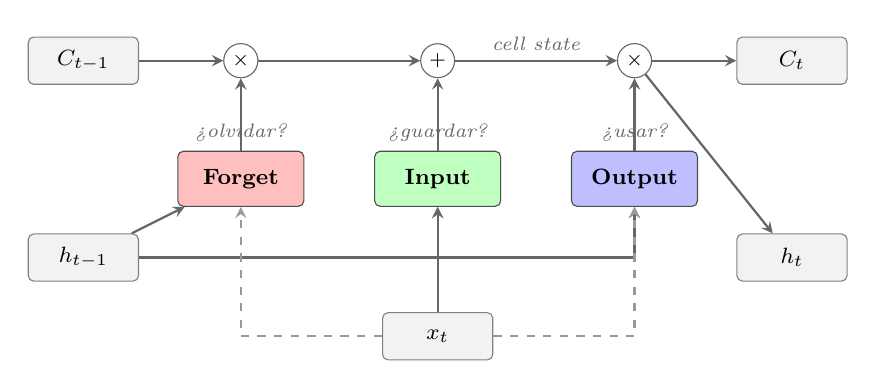
\begin{tikzpicture}[
  gate/.style={rectangle, draw=black!70, fill=#1!25, minimum width=1.6cm,
    minimum height=0.7cm, rounded corners=2pt, font=\footnotesize\bfseries, text centered},
  state/.style={rectangle, draw=black!50, fill=gray!10, minimum width=1.4cm,
    minimum height=0.6cm, rounded corners=2pt, font=\footnotesize},
  op/.style={circle, draw=black!60, fill=white, inner sep=1.5pt, font=\scriptsize},
  arr/.style={->, >=stealth, thick, draw=black!60},
  lbl/.style={font=\scriptsize\itshape, text=black!60}
]
  % Puertas
  \node[gate=red]    (fg) at (0,0)   {Forget};
  \node[gate=green]  (ig) at (2.5,0) {Input};
  \node[gate=blue]   (og) at (5,0)   {Output};
  % Operaciones
  \node[op] (mul1) at (0,1.5)   {$\times$};
  \node[op] (mul2) at (2.5,1.5) {$+$};
  \node[op] (mul3) at (5,1.5)   {$\times$};
  % Estados
  \node[state] (ct1) at (-2,1.5)  {$C_{t-1}$};
  \node[state] (ct)  at (7,1.5)   {$C_t$};
  \node[state] (ht1) at (-2,-1)   {$h_{t-1}$};
  \node[state] (ht)  at (7,-1)    {$h_t$};
  % Entrada
  \node[state] (xt)  at (2.5,-2)  {$x_t$};
  % Conexiones del cell state
  \draw[arr] (ct1) -- (mul1);
  \draw[arr] (mul1) -- (mul2);
  \draw[arr] (mul2) -- node[above, lbl]{cell state} (mul3);
  \draw[arr] (mul3) -- (ct);
  % Puertas a operaciones
  \draw[arr] (fg) -- (mul1);
  \draw[arr] (ig) -- (mul2);
  \draw[arr] (og) -- (mul3);
  % Hidden state y entrada a puertas
  \draw[arr] (ht1) -- (fg);
  \draw[arr] (ht1) -| (ig);
  \draw[arr] (ht1) -| (og);
  \draw[arr] (xt) -- (ig);
  \draw[arr, dashed, black!40] (xt) -| (fg);
  \draw[arr, dashed, black!40] (xt) -| (og);
  % Salida h_t
  \draw[arr] (mul3) -- (ht);
  % Etiquetas
  \node[lbl, above] at (fg.north) {¿olvidar?};
  \node[lbl, above] at (ig.north) {¿guardar?};
  \node[lbl, above] at (og.north) {¿usar?};
\end{tikzpicture}
\caption{Estructura de una celda LSTM con sus tres puertas de control.}
\label{fig:lstm_cell}
\end{figure}

La \textbf{puerta de olvido} decide qué información del estado anterior descartar, permitiendo ``olvidar'' contexto irrelevante. La \textbf{puerta de entrada} controla qué nueva información incorporar al estado. La \textbf{puerta de salida} determina qué parte del estado usar para la predicción actual. Este mecanismo permite a las LSTM mantener información relevante durante cientos de pasos temporales, lo que las hace especialmente adecuadas para series financieras donde eventos pasados pueden tener efectos persistentes.

Se utilizaron dos capas apiladas con 50 unidades cada una, dropout del 20\% para regularizar, y una capa densa final. El entrenamiento se realiza con Adam y pérdida MSE.

\subsubsection{GRU (Gated Recurrent Units)}

Las GRU~\cite{cho2014learning} representan una simplificación de las LSTM. Combinan las puertas de olvido y entrada en una única \textbf{puerta de actualización} (update gate), y añaden una \textbf{puerta de reset} que controla cuánto del estado anterior considerar. Esta simplificación reduce el número de parámetros aproximadamente en un 25\%, lo que acelera el entrenamiento y puede reducir el sobreajuste en datasets pequeños.

En la práctica, GRU suele dar resultados comparables a LSTM en muchas tareas, y en algunos casos los supera precisamente por su menor propensión al sobreajuste. Se utilizó la misma arquitectura básica que LSTM: dos capas con 50 unidades y dropout del 20\%.

\subsubsection{CNN 1D (Convolutional Neural Network)}

Las CNN unidimensionales aplican filtros convolucionales sobre la secuencia temporal. A diferencia de las arquitecturas recurrentes, las CNN no tienen memoria explícita: procesan la secuencia como un bloque y detectan patrones locales mediante los filtros.

Se utilizaron filtros de tamaño 2 para detectar patrones de 2 días consecutivos. La ventaja de las CNN es su velocidad de entrenamiento y su capacidad para capturar patrones locales de forma eficiente. Su limitación es que no modelan dependencias de largo plazo tan bien como las recurrentes, lo que puede ser problemático en series con estructura temporal compleja.

\subsection{Configuración común}

Para todos los modelos deep learning, la entrada es una ventana de 30 días con las características escaladas entre 0 y 1. El MinMaxScaler se ajusta solo con los datos de entrenamiento y luego se aplica al test para evitar fuga de información. Además, se excluyen explícitamente las columnas \texttt{Target\_*}, ya que se calculan con \texttt{shift(-h)} y contienen información futura.

\section{Evaluación de los modelos}

Evaluar modelos de series temporales presenta particularidades relevantes. La validación cruzada clásica no es aplicable porque mezclaría pasado y futuro, violando la causalidad temporal y dando resultados inflados~\cite{hyndman2021forecasting}.

Se utilizó en su lugar \textbf{validación walk-forward}, que replica cómo funcionaría el modelo en el mundo real. La Figura~\ref{fig:walkforward} muestra el esquema.

\begin{figure}[H]
\centering
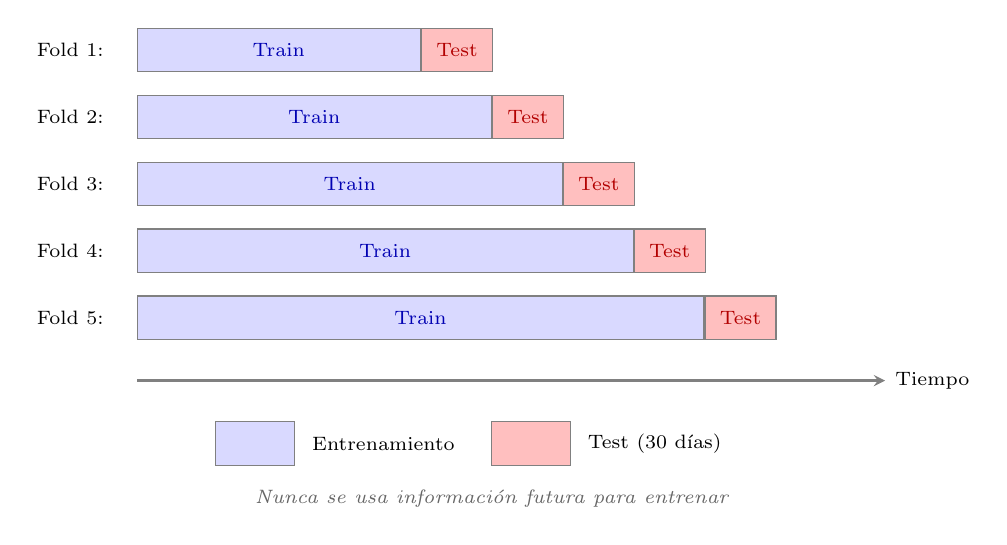
\begin{tikzpicture}[
  train/.style={rectangle, draw=black!50, fill=blue!15, minimum height=0.55cm, font=\scriptsize},
  test/.style={rectangle, draw=black!50, fill=red!25, minimum height=0.55cm, font=\scriptsize},
  lbl/.style={font=\scriptsize, anchor=east},
  arr/.style={->, >=stealth, thick, draw=black!50}
]
  \foreach \i/\tlen/\tstart in {1/4/4, 2/5/5, 3/6/6, 4/7/7, 5/8/8} {
    \pgfmathsetmacro{\y}{-(\i-1)*0.85}
    \pgfmathsetmacro{\testx}{\tlen*0.45 + \tlen*0.45}
    \node[lbl] at (-0.3, \y) {Fold \i:};
    \node[train, minimum width=\tlen*0.9 cm] (tr\i) at (\tlen*0.45, \y) {\textcolor{blue!70!black}{Train}};
    \node[test, minimum width=0.9cm, anchor=west] (te\i) at (tr\i.east) {\textcolor{red!70!black}{Test}};
  }
  % Flecha temporal
  \draw[arr] (0,-4.2) -- (9.5,-4.2) node[right, font=\scriptsize] {Tiempo};
  % Leyenda
  \node[train, minimum width=1cm] at (1.5,-5) {};
  \node[font=\scriptsize, right] at (2.1,-5) {Entrenamiento};
  \node[test, minimum width=1cm] at (5,-5) {};
  \node[font=\scriptsize, right] at (5.6,-5) {Test (30 días)};
  % Nota
  \node[font=\scriptsize\itshape, text=black!60] at (4.5,-5.7) {Nunca se usa información futura para entrenar};
\end{tikzpicture}
\caption{Esquema simplificado de la validación walk-forward (cinco de las doce iteraciones utilizadas).}
\label{fig:walkforward}
\end{figure}

La mecánica es intuitiva: se entrena con todo lo que hay hasta cierto punto, se predice el bloque siguiente, se avanza el punto de corte y se repite. Al cabo de doce iteraciones se tiene una estimación bastante más fiable que con un único train/test.

Un matiz importante: el bloque de test tiene 30 días (\texttt{test\_size=30}) porque se necesitan varias observaciones para medir el rendimiento, pero el horizonte de predicción se mantiene fijo. En cada fold se generan 30 predicciones, una por cada fecha $t$ del bloque, y cada predicción estima directamente $t+h$ usando únicamente datos reales disponibles hasta $t$. No se encadenan predicciones ni se sustituyen datos reales por predicciones; es un esquema de origen móvil. Por eso las curvas de predicción aparecen continuas incluso cuando $h=7$. En acciones, estos ``días'' corresponden a \textbf{sesiones de mercado} (no hay fines de semana en la serie); en BTC-USD sí hay datos diarios incluyendo fines de semana. En los modelos tabulares (Random Forest y XGBoost), para evitar fuga en los límites de cada fold se excluyen del entrenamiento las últimas $h$ observaciones del bloque de train, ya que su objetivo depende de precios que caen dentro del bloque de test. En ARIMA también se evita reentrenar dentro del bloque de test: se ajusta una vez por fold y después solo se actualiza el estado con observaciones nuevas (sin \textit{refit} de parámetros).

Para asegurar reproducibilidad, se fijó una semilla global en todas las ejecuciones de entrenamiento y evaluación, y se reinicia al inicio de cada entrenamiento (por fold y modelo).

Las métricas calculadas son RMSE, MAE y MAPE~\cite{hyndman2006another}, además de métricas direccionales (MDA, F1 y MCC). El análisis se centra en el MAPE porque expresa el error como porcentaje, lo que facilita la comparación entre activos de distinta escala. Un MAPE del 3\% indica que, en promedio, el error absoluto es del orden del 3\% del precio real. Todas las métricas finales se reportan sobre el precio futuro (no sobre retornos), lo que mantiene una interpretación directa en dólares.

\section{Estudio de ablación}

Un \textbf{estudio de ablación} consiste en eliminar un componente del sistema y evaluar el efecto sobre el rendimiento. Es una técnica habitual en aprendizaje automático para aislar la contribución de cada componente. En este trabajo se emplea para determinar si el sentimiento contribuye positivamente a la predicción o introduce ruido.

Para ello, se ejecutan los mismos modelos de deep learning dos veces: una con la variable de sentimiento incluida y otra sin ella. La comparación de los errores entre ambas configuraciones permite aislar el efecto del sentimiento.

Si eliminar el sentimiento empeora las predicciones de forma consistente, se obtiene evidencia de que aporta información que los modelos pueden explotar. Si no se observa diferencia, no habría evidencia de señal útil bajo este conjunto de datos, modelos y protocolo.

Para evaluar esa diferencia con mayor rigor, se aplica un \textbf{test de Wilcoxon pareado} sobre las métricas por fold. De esta forma no solo se comparan medias, sino que se verifica si el efecto del sentimiento es estadísticamente consistente.

También se compara el rendimiento de los tres modelos DL en distintos periodos de mercado: el rally alcista de 2021, el mercado bajista de 2022, y el periodo más reciente. El objetivo es determinar si las arquitecturas se comportan de forma similar en todos los contextos o si alguna falla ---o destaca--- en condiciones específicas.

\section{Más allá del error: métricas complementarias}

El MAPE resulta útil para la comparación entre modelos, pero no refleja todos los aspectos del rendimiento predictivo. Que un modelo tenga un error porcentual bajo no significa que sirva para tomar decisiones de inversión. Se añadieron dos métricas que aportan un poco más de perspectiva.

\subsection{Precisión direccional}

La \textbf{precisión direccional} (\textit{Directional Accuracy}) mide el porcentaje de veces que el modelo acierta si el precio futuro sube o baja respecto al precio de origen. Esta métrica es útil para interpretar el valor potencial del modelo en contextos de decisión, donde el signo del movimiento puede ser más relevante que el nivel exacto.

Matemáticamente, en un horizonte $h$, si $y_t$ es el precio observado en la fecha de origen y $\hat{y}_{t+h}$ es la predicción del precio futuro, la precisión direccional compara el signo del cambio a $h$ días:

\[
\text{DA}_h = \frac{1}{n} \sum_{t=1}^{n} \mathbf{1}[\text{sign}(y_{t+h} - y_t) = \text{sign}(\hat{y}_{t+h} - y_t)]
\]

En este trabajo se utiliza esta definición contra el precio de origen ($y_t$) porque las predicciones son directas a $t+h$ (no se encadenan). Un modelo que acierta en torno al 50\% de las direcciones no mejora al azar. Solo si supera de forma consistente ese umbral podría considerarse que existe señal predictiva direccional.

Además de la tasa de acierto bruta, se calculan dos métricas complementarias: el \textbf{F1 direccional}, que está centrado en la clase ``sube'' y tiene en cuenta tanto precisión como recall, y el \textbf{MCC} (Matthews Correlation Coefficient), que penaliza de forma más equilibrada los errores cuando hay asimetrías entre subidas y bajadas. Estas métricas son especialmente útiles cuando las clases están desbalanceadas, como suele ocurrir en mercados con tendencias marcadas.

\subsection{El test de Diebold-Mariano}

Cuando se comparan dos modelos y uno presenta un MAPE ligeramente menor, es necesario determinar si la diferencia es robusta o compatible con variabilidad muestral. El \textbf{test de Diebold-Mariano}~\cite{diebold1995comparing} permite contrastar formalmente esta hipótesis.

La idea es comparar las pérdidas (por ejemplo, errores al cuadrado) de dos modelos a lo largo del tiempo y evaluar si la diferencia media es estadísticamente significativa. En este trabajo se adopta un umbral de significancia del 5\%. En la implementación se utiliza la corrección de Harvey, Leybourne y Newbold~\cite{harvey1997testing}, que emplea una distribución t-Student para muestras finitas.

En los resultados principales se ejecuta el test con horizonte $h=7$, para que el ajuste de autocovarianzas sea coherente con el horizonte de predicción utilizado en los experimentos (independiente de que el bloque de test por fold tenga 30 días). Este test es especialmente relevante para comparar modelos sofisticados contra el baseline Naive: si la mejora de un modelo sobre Naive no es estadísticamente significativa, toda la complejidad adicional no estaría aportando valor real y sería preferible optar por la solución más simple.
